\documentclass[a4paper,12pt]{article}

\usepackage[pdftex]{graphicx}

\begin{document}

\title{Senior Project Report: Localization, Mapping and Path-Planning for Inexpensive Robots}
\author{Austin Hendrix}
\date{May 2011}
\maketitle

\section{Abstract}
This project aims to create a small mobile robot that is capable of accurate localization, path-planning and obstacle avoidance, and to compete in Sparkfun's autonomous vehicle competition\cite{avc}. Localization, path-planning and obstacle avoidance are important for mobile robots because they allow the construction of more complex and useful behaviors. I was able to achieve the goal of building a reliable robot capable of good obstacle avoidance and rudimentary navigation, but I didn't have time to achieve accurate localization or a map suitable for path-planning.

\begin{figure}
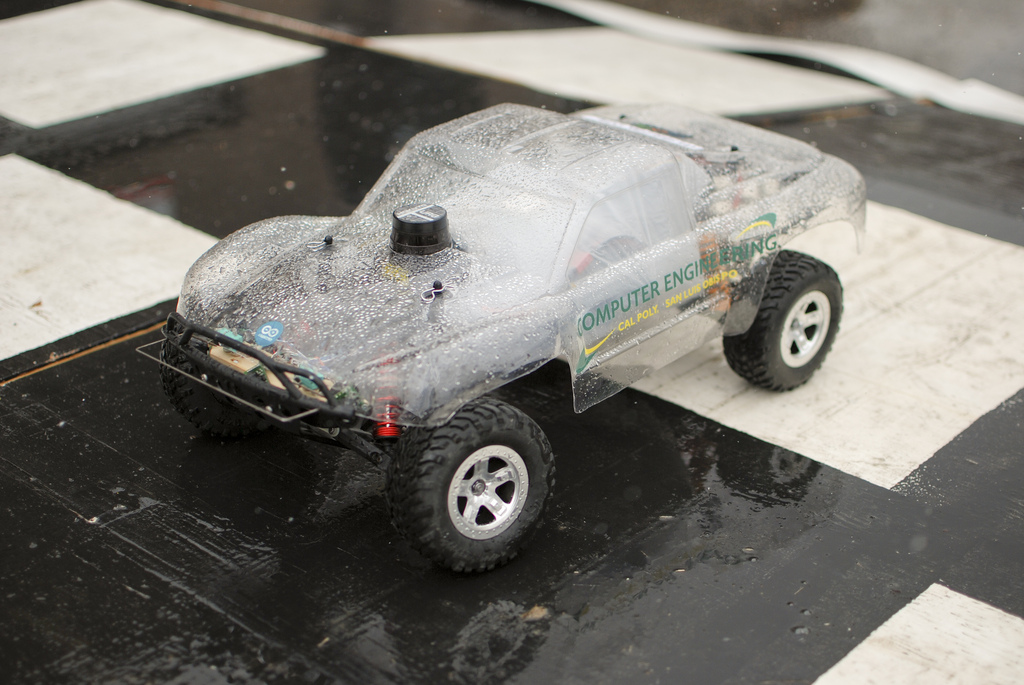
\includegraphics[width=1.00\textwidth]{start}
\caption{At Sparkfun AVC, on the starting line}
\end{figure}

\section{Background}
\subsection{Software}
Localization, path-planning and obstacle avoidance have been studied in mobile robots since Stanford created Shakey\cite{shakey}. Most of the research and techniques for this project come from "Probabilistic Robotics,"\cite{thrun} but are focused primarily on indoor applications. Techniques used include proportional control for speed regulation and Kalman filtering to fuse GPS, odometry and compass data. Since all of the hardware was new at the start of this project, there was no initial software; all software was written during the course of the project.

\subsection{Hardware}
The platform for this project is a robot that the author has been working on for a number of years. It consists of a modified 1/8 scale RC car (Traxxas Slash\cite{traxxas}), with three forward-facing and two rear-facing sonar distance sensors, a front bump sensor, wheel encoders, a GPS, a compass, a serial Bluetooth module, an Arduino Mega 2560 microcontroller, a single-board computer with a 500MHz processor running Linux, and a Hokuyo URG-04LX-UG01 scanning laser range finder. The chassis has been modified, with an upgraded motor, motor controller and suspension better suited for robotics. This platform has proven to be reliable and robust in past projects.

\section{Problem Statement}
For my senior project, I built and programmed a relatively inexpensive robot to perform localization, mapping and path-planning. The purpose of this project was to explore the capabilities of a relatively low-cost, semi-autonomous robot, and to explore the capabilities of open-source robotics software. The robot was intended to compete in the SparkFun Autonomous Vehicle Competition\cite{avc}, and to be able to navigate around Cal Poly's Inner Perimeter Road, given a reasonable number of intermediate GPS coordinates. In general, no assumptions were made about the size of the world that the robot would operate in. Since the robot was intended to operate outdoors, is was assumed that most obstacles would be large (\textgreater10cm) and tall enough to be seen by the scanning laser range finder, or short enough to be driven over.

\section{Design}
\subsection{Hardware Selection}

After significant development of this platform for a previous class, I came to the conclusion that it needed some significant hardware redesign to accomplish my goals of outdoor SLAM and navigation. In particular, it needed more and more accurate range measurements of its environment, and it needed a more powerful onboard processor and a more unified architecture.

To these ends, I selected a Hokuyo URG-04LX-UG01 scanning laser range finder as the appropriate sensor. I also considered other scanning laser range finders and the Microsoft Kinect; the other lasers were more expensive, heavier, and required more power than the Hokuyo model I chose, and the Kinect was larger, heavier, used more power, and would have required a dedicated power supply to convert the robot's 8.4V battery to the 12V required by the Kinect.

The sensor selection dictated that the onboard computer needed to have host USB support, which limited my selection to a small number of embedded systems motherboards, small form-factor motherboards and the arm-based gumstix boards. Most of the small form-factor motherboards required a 12V ATX power connector to supply power, and those that didn't required a single 12V input, which would again require a separate boost convertor. The gumstix boards met most of my specifications, but have only 1 USB host port, and are difficult to expand. The embedded systems board that I found was an ALIX 3d2, which accepts a 7-20V input voltage, nearly perfectly matched to my batteries, has two USB host ports, and as a bonus has a TTL-level serial port on board, which eliminates the need for level-conversion when communicating between it and a 5V microcontroller. The ALIX is smaller than most small form-factor motherboards, and significantly larger than the gumstix, but was still of a size that was feasible to fit on the robot. I chose the ALIX and proceeded to microcontroller selection.

The requirements for my microcontroller were fairly strict; I needed at least 3 hardware UARTS, for communication with my GPS, sonars and the primary computer. An ideal microcontroller would have a 4th UART for communicating with the bluetooth serial module for external control. It also needed a significant number of digital I/O lines for reading the wheel sensors, bump sensor, and controlling the sonars, and a few analog inputs for reading the battery voltages. I considered the parallax propeller, the AtMega2560-based Arduino mega, and the Digilent Nexys II development board. The propeller meets all of the functional requirements, but from previous experience I knew that the development environment was windows-only, and diffcult for me to work with. The Arduino Mega met all of the functional requirements, and has a strong open-source tool chain that works on all major platforms. The Digilent Nexys II, being FPGA-based rather than a microtontroller, far exceeded all of the funtional requirements, but the development environment is also windows-only, and it requires significantly more development time than an equivalnet microcontroller to achieve the same results. I select the Arduino Mega because it met all of my requirements, and had a strong open-source toolchain.

I retained all of my existing sensors and interfaced them to the Arduino, including 4 wheel position sensors, 3 front sonars, 2 rear sonars, a front bump sensor, a GPS, and a compass.


\subsection{Budget}
\begin{tabular}{lr}
Hokuyo URG-04LX-UG01: & \$1200 \\
ALIX 3D2 Single-board computer: & \$125 \\
Parallax GPS: & \$80 \\
Bluetooth Modem: & \$65 \\ 
Arduino Mega 2560: & \$65 \\ 
HM55B Compass: & \$30 \\ 
Traxxas Slash (2WD): & \$377 \\ 
5x MaxSonar EZ1: & \$114 \\
Spare Batteries: & \$113 \\
Misc: & ~\$100 \\
\hline
Total: & \$2269
\end{tabular}

\subsection{Software Design}
The system has the following custom ROS nodes:
\begin{itemize}
   \item Hardware interface
   \item Goal list
   \item gps\_odometry: kalman filter
   \item global map server
   \item path planner
\end{itemize}
And the following stock nodes:
\begin{itemize}
   \item gpsd\_client
   \item laser driver
\end{itemize}




\section{Implementation}
\subsection{Hardware}

\begin{figure}[h!]
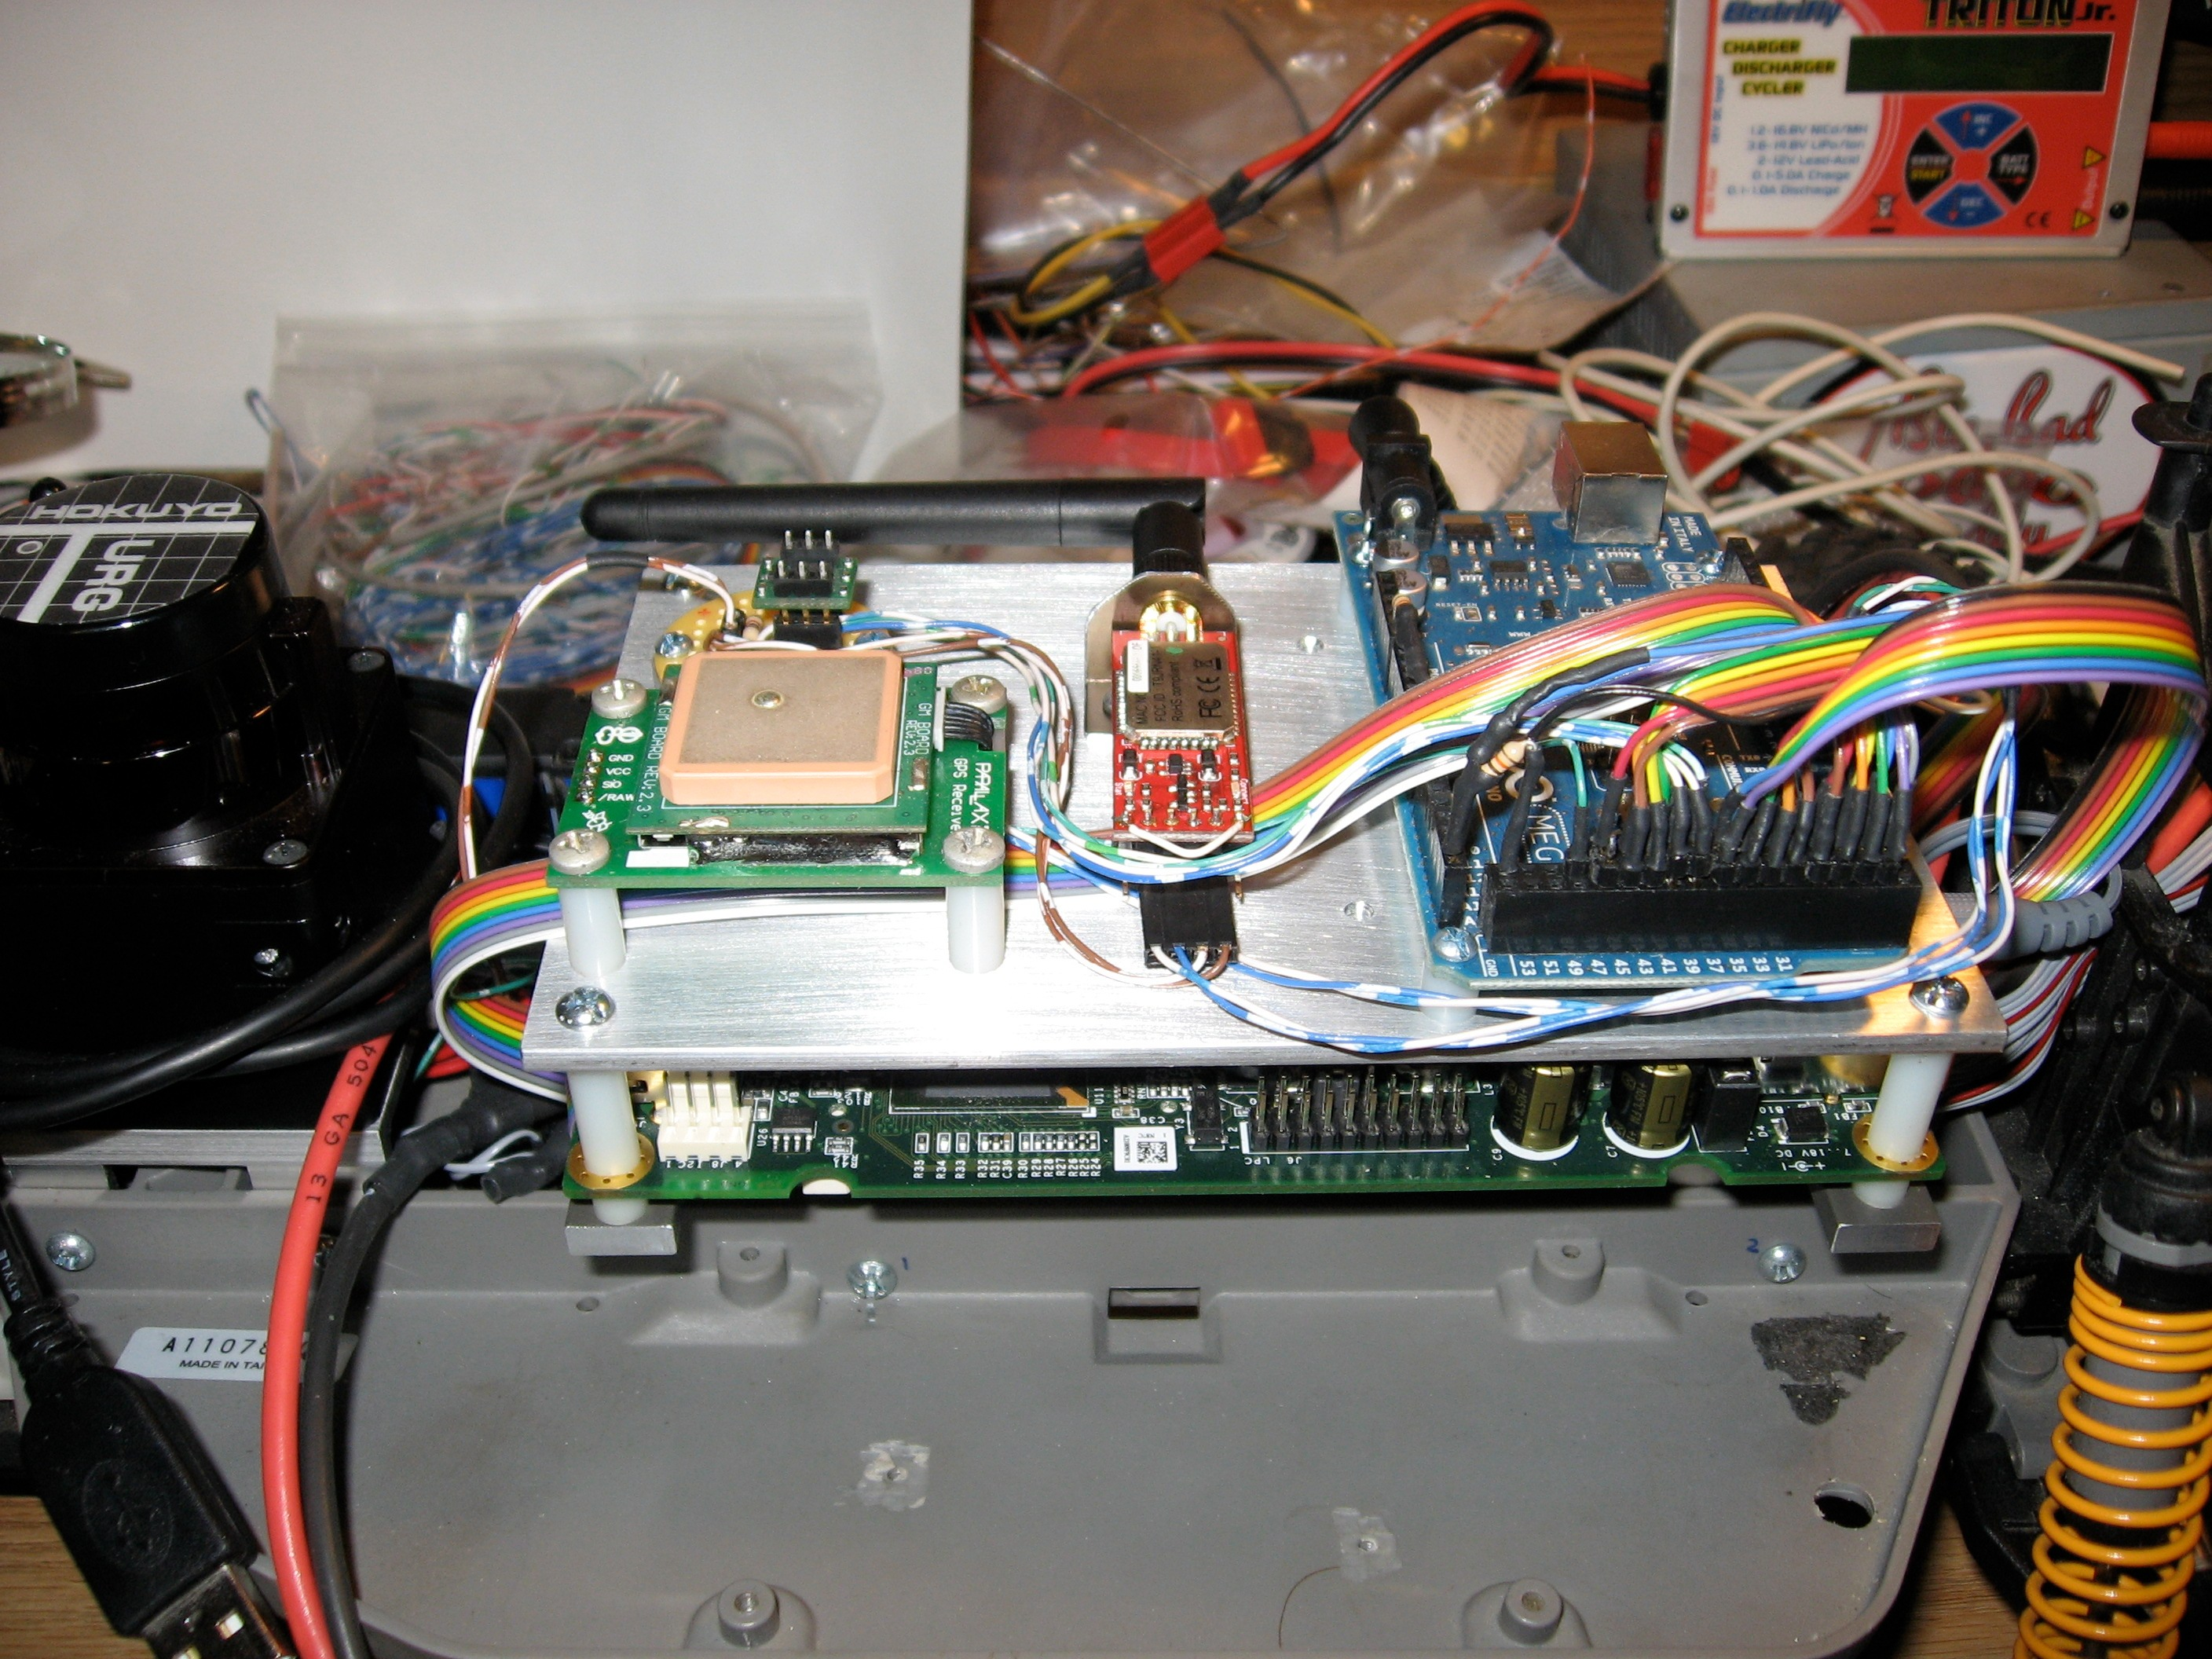
\includegraphics[width=1.0\textwidth]{hardware}
\caption{Internals and sensors}
\end{figure}

I replaced the original wiring and interface circuitry, built from whatever components I had lying around, stuck into a breadboard, with properly selected componenets on a custom perfboard, with color-coded wiring.

I also replaced the original RC motor controller, which had problems switching into reverse, with a motor driver from pololu, driven with PWM generated on the arduino.

The power distribution system consists of two batteries, allowing me to isolate the motor supply from the electronics supply, while sharing a common ground. This provides enough noise isolation that the electronics are unaffected by noise from the motor, which had been a problem in the past.

The sensors are powered by a switching 5V regulator, while the arduino and the primary computer are connected directly to the battery supply voltage. There is also an electonic power cutoff, allowing the electonics to shut off automatically to avoid running the batteries too low. The 5V regulator has an enable line, allowing the sensors to be turned off, should the need arise.


\subsection{Firmware}

The firmware on the arduino is based on a real-time OS that I wrote for the previous atmega controller that ran this robot. 
The RTOS core provides basic preemptive multitasking and interval scheduling, and process priorities. Each process runs until it is either preempted, or it calls the yeild() function to indicate that it is done processing until its timer expires. This requires some careful process design on the part of the programmer, but makes the task switcher and the scheduler simple and fast, with an overhead of about 1-2\% at an interrupt rate of 1000Hz.
A simple locking library provides semaphors for controlling access to shared resources, since the processor doesn't provide native semaphors or memory access protection.
Driver libraries provide interrupt routines, buffers and access functions to interface with the A2D converter, hardware UARTs, compass, and motor and servo PWM.

There are threads within this RTOS for:
\begin{itemize}
   \item Polling the wheel eoncders and computing the speed/direction
   \item Controlling the motor power to achieve a constant speed
   \item Reading data from the GPS and transmitting it to the primary computer
   \item Reading and interpreting command data from the bluetooth interface
   \item Reading and interpreting command data from the primary computer
   \item Peridocally sending odometry, compass and battery data to the primary computer
   \item counting idle cycles (the idle task, runs when nothing else is running)
\end{itemize}

With proper tuning, this worked very well, but still experienced occasional lockups of unknown origin.


\subsection{Software}

\begin{figure}
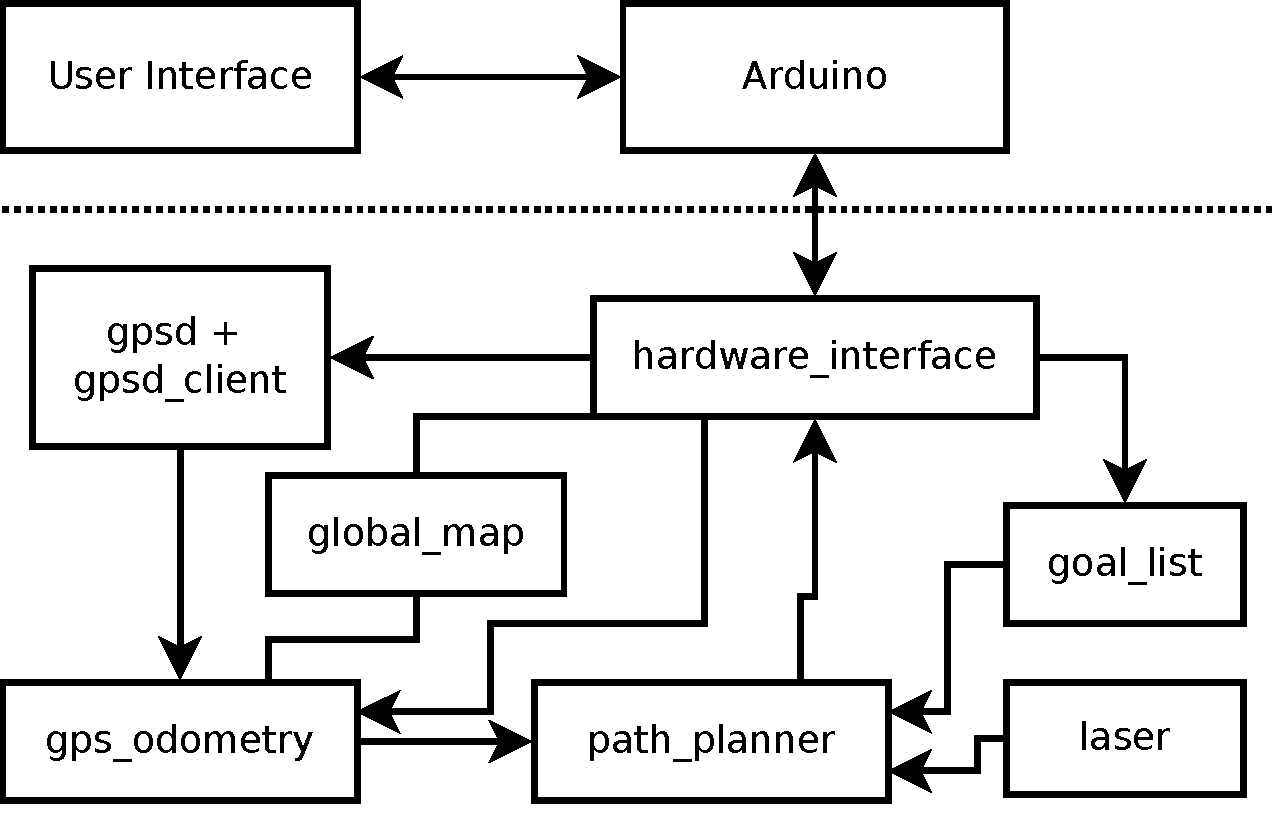
\includegraphics[width=1\textwidth]{software_flow}
\caption{Software Architecture}
\end{figure}

The primary computer runs Gentoo, a Linux distribution, and runs the ROS software package to support the high-level behaviors. Each behavior or part of the system is implemented as a separate ROS node, and communicates with other nodes through messages or service calls.

The \texttt{hardware\_interface} node is responsible for translating data from the Arduino into ROS messages, and for translating some ROS messages into control and status data to be sent to the Arduino. 

The \texttt{hardware\_interface} node recieves odometry, bump sensor, battery level, GPS, and compass data from the Arduino. It translates the odometry data into odometry messages, using a kinematic model of the robot to translate encoder counts and wheel movements into position change in x, y, and heading. It translates the compass data (really an x-y magnetometer) into a heading from north, and publishes that angle in a compass message. It takes the GPS data, as NMEA strings, and sends it to an instance of gpsd\cite{gpsd}, which parses the data, and publishes it, to be read by the \texttt{gpsd\_client} node, which publishes the resulting data as GPSFix messages. It records the battey level data into a log file, for later analysis; eventually, this data will be used to build a model to predict remaining battery capacity. It ignores the bump sensor data. The \texttt{hardware\_interface} node also receives a list of gps coordinates that is forwarded through the Arduino from the user interface, and publishes this as a GoalList message.

The \texttt{hardware\_interface} node recieves command messages as speed and steering commands, and transmits them to the Arduino. It also recieves position estimate messages, translates them into GPS coordinates, and transmits them to the Arduino, to be forwarded to the user interface.

The \texttt{global\_map} node is responsible for storing the map, and for the mapping of GPS coordinates to map coordinates. It uses a transverse mercator projection to map latitude/longitude coordinates onto a square grid. It chooses the nearest longitude line, to the nearest degree, to use as the local meridian for the projection. This makes it easy to choose a meridian based on the current position, it allows GPS coordinates to be mapped onto a square grid, and it minimizes the distortion when translating from one coordinate system to the other. The \texttt{global\_map} node provides a pair of ROS Services that map GPS coordinates to row/column addresses in the map, and from row/column addresses back to GPS coordinates.

The \texttt{goal\_list} node is responsible for maintaining the list of goals from the user, and for tracking which goal is the current goal. It receives new lists of goals from the \texttt{hardware\_interface}, and the current position of the robot, and publishes the current goal. It considers a goal to be reached when it is within a pre-configured distance, and moves on to the next goal.

The \texttt{gps\_odometry} node is responsible for performing Kalman filtering to fuse GPS, compass and odometry data to produce a more accurate position estimate. It's implemented as two kalman filters; one for row/column position in map coordinates, and separate filter for heading. This was possible because there is no correlation between the robot's heading and its position; it allows for simpler update steps and smaller covariance matrices. Updates are done whenever new data arrives, based on the type of the data. Odometry is treated as a prediction update, while compass and GPS data is treated as measurement updates.

The \texttt{path\_planner} node is responsible for directing the robot from its current position to the current goal position while avoiding obstacles. It receives the position of the robot, the current goal, and laser scan data, and publishes steering and speed commands to the \texttt{hardware\_interface}. It is implemented as reactive goal follower with obstacle avoidance; it computes the desired heading to the goal based on the robot's position, then checks to see that this heading is obstacle-free, based on the most recent scan from the laser. If it isn't, it searches headings to either side of the desired heading until it finds one that is obstacle free. It uses this heading to compute the desired change in heading, and uses that to proportionally control the steering. It sets a constant forward speed.

The laser node is a stock ROS node (\texttt{hokuyo\_node}) that reads data from the laser over USB, and publishes it as a ROS message.


\subsection{User Interface}

While not directly related to the functionality of the robot, a good user interface makes it much easier to interact with, control and view debugging information from the robot. To that end, I used a Motorola Xoom tablet computer communicating over bluetooth the control the robot. The user interface consisted of a touchable map interface, using data from Google Maps, that reported the position of the user, the estimated position of the robot, and allowed the user to control the robot, via direct control of the motors or by supplying the robot with a series of GPS points to follow, by touching the map.


\section{Testing}
The first round of testing was to ensure that the odometry was working properly; the first data set is the location dereived solely from odometry data.

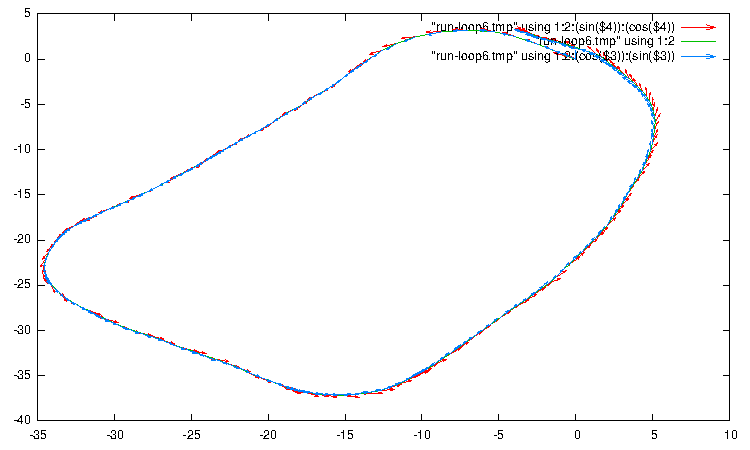
\includegraphics{run-loop6}


TODO: Gather lots of data about the robot performance and makes some pretty graphs of it.

\section{Conclusions}

\section{Final Thoughts}

Due to tight time constraints before the competition, made worse by unforseen circumstances, I decided to drop a true path-planning algorithm and instead focus on a reactive approach to avoiding obstacles and following waypoints. The main problem with my A* algorithm was that it took too many iterations to run, and had to re-plan too often. I replaced it with an algorithm that computed the heading to the target, checked for obstacles along that path and at increasing deviations from that path until a collision-free heading was found, and then set the steering angle based on the difference between that target angle and the robot's current heading. This proved quite effective at avoiding obstacles that were directly ahead of the robot, but surprisingly less well at avoiding obstacles to the left or right of the robot.

( code thoughts:
  probably caused by partial visibility of lidar combined with a target angle near +/- pi/2; the robot thinks that things outside of the front arc are clear, and picks a target angle that points backward
  TODO:
   consider the true path the robot will follow rather than assuming a straight line
   if all paths forward are blocked, consider a path backward
   keep a local obstacle map so that the robot has some idea of what is behind it
   )

After talking with the competition winner, it's obvious that the key to his success was twofold: good software design and lots of testing; from what I heard, he spent at least as long testing and tuning his algorithm as he did designing and writing the algorithm. This definitely showed in his final product, and points out the flaws in my process: I think that if I had spent more time testing and tuning my kalman filter, I would have been able to at least make it all the way around the building.

TODO: do the proper test runs and gather data that supports that a) my current turning of my kalman filter sucks and b) tune the kalman filter properly.

Another problem that arose during competition was the robot's inability to detect curbs. This wasn't a huge issue, because the robot was generally able to climb any curb it couldn't see; however, the ability to detect and avoid curbs would have given the robot a better chance of successfully completing the competition.


\section{References}
\begin{thebibliography}{9}

\bibitem{thrun}
   Sebatian Thrun, et al.
   \emph{Probabilistic Robotics}
   The MIT Press, Massachusetts
   2006.

\bibitem{traxxas}
   Traxxas Slash (2wd)
   \textless{}http://traxxas.com/products/models/electric/5805slash\textgreater

\bibitem{shakey}
   \uline{AI Center::Shakey}. SRI International: Artificial Intelligence Center
   \textless{}http://www.ai.sri.com/shakey/\textgreater

\bibitem{avc}
   SparkFun Autonomous Vehicle Competition
   \textless{}http://www.sparkfun.com/products/10435/\textgreater

\bibitem{gpsd}
   GPSd
   \textless{}http://gpsd.berlios.de/\textgreater

\end{thebibliography}


\section{TODO}
\input{todo}

\section{misc}
I propose to write software to control this robot; by the end of the quarter I would like to be able to map and navigate indoor and outdoor spaces. In an indoor space, the robot should be able to navigate to a set of coordinates relative to its initial starting position. In an outdoor space, the robot should be able to navigate to a GPS location, within the limits of GPS accuracy. An ideal end-of-quarter demonstration would be to navigate Cal Poly's Inner Perimeter road, given a sufficient number of intermediate GPS coordinates and none or light foot traffic. Algorithms for accomplishing this will probably include Kalman filters to smooth the input data, some sort of compass calibration and offset algorithm to compensate for nearby metal objects, and a map based on a fine occupancy grid, since the robot will be expected to operate in unstructured environments. Open-source robotics software will be used where possible to speed up development. 

The robot should be mostly autonomous, aside from high-level motion commands in the form of target destinations, in absolute or relative coordinates, for the robot to navigate to. Commands with either be pre-programmed, or transmitted to the robot over a wireless link.

Potential avenues of investigation once navigation and planning have been achieved to a reasonable degree include mounting a Kinect to the robot to explore its capabilities, or mounting a USB nerf turret with a webcam to the robot, allowing it to find, track, follow and shoot targets of the operator's choosing.

\end{document}
